% ============================================================================
% chapitre4.tex — Realisation
% ============================================================================
\chapter{Realisation}
\label{chap:realisation}

\introchapitre

Ce dernier chapitre presente la realisation effective du systeme conçu dans le
chapitre precedent. Nous decrivons d'abord l'environnement materiel et logiciel mis
en place, puis nous illustrons le fonctionnement du pipeline a travers les principales
interfaces graphiques produites par chaque composant.

\section{Environnement de developpement}
\label{sec:env}

\subsection{Environnement materiel et logiciel}

L'environnement de developpement local repose sur \textbf{WSL2} (Windows Subsystem for
Linux 2) avec Ubuntu, sur lequel est deploye un cluster \textbf{Minikube} (pilote
Docker, 6~vCPU, 6~Go de RAM). Cette configuration permet d'executer l'ensemble du
cluster Kubernetes --- Kafka, Flink, MinIO, PostgreSQL, Prometheus et Grafana --- sur
une seule machine de developpement, sans dependance a une infrastructure cloud.

\begin{table}[H]
\centering
\renewcommand{\arraystretch}{1.5}
\begin{tabular}{|l|l|p{7.3cm}|}
\hline
\textbf{Outil} & \textbf{Version} & \textbf{Role dans le projet} \\
\hline
Minikube & 1.38.1 & Cluster Kubernetes local (pilote Docker, 6 vCPU / 6 Go RAM) \\
kubectl & $\geq$ 1.28 & CLI Kubernetes pour la gestion des pods et services \\
Helm & $\geq$ 3.12 & Gestionnaire de paquets Kubernetes (Strimzi, MinIO) \\
Terraform & $\geq$ 1.0 & Infrastructure as Code --- provisionne l'ensemble des ressources \\
Strimzi Operator & 0.51.0 & Operateur Kubernetes pour Apache Kafka (mode KRaft) \\
Apache Kafka & 4.1.0 & Bus d'evenements distribue \\
Apache Flink (PyFlink) & 1.19.1 & Traitement de flux en continu \\
PostgreSQL & 15 / 16 & Persistance finale (\texttt{gold\_transactions}) \\
Python & 3.11 & Langage des jobs Flink, scripts producteur et exporteur \\
Docker & $\geq$ 24.0 & Moteur de conteneurs \\
\hline
\end{tabular}
\caption{Environnement logiciel du projet}
\label{tab:outils}
\end{table}

\begin{table}[H]
\centering
\renewcommand{\arraystretch}{1.5}
\begin{tabular}{|l|l|p{7.6cm}|}
\hline
\textbf{Bibliotheque} & \textbf{Version} & \textbf{Role} \\
\hline
\texttt{apache-flink} & 1.19.1 & API PyFlink pour les quatre jobs de streaming \\
\texttt{cryptography} & $\geq$ 41.0 & Chiffrement Fernet (AES-128-CBC + HMAC-SHA256) \\
\texttt{minio} & $\geq$ 7.2 & Client SDK MinIO/S3 pour l'ecriture Medallion \\
\texttt{kafka-python} & 2.0.2 / 2.3.1 & Producteur et composants Python (gold-flattener, gold-sink) \\
\texttt{pandas} & $\geq$ 2.0 & Lecture des fichiers CSV source \\
\texttt{psycopg2-binary} & $\geq$ 2.9 & Connecteur PostgreSQL \\
\texttt{prometheus\_client} & $\geq$ 0.20 & Exposition des metriques metier personnalisees \\
\hline
\end{tabular}
\caption{Bibliotheques Python utilisees}
\label{tab:libs}
\end{table}

\textit{Note technique :} l'image \texttt{python:3.11-slim} a ete retenue pour tous
les composants Python conteneurises du pipeline (\texttt{gold-flattener},
\texttt{gold-sink}) ; la version 3.12 a ete ecartee apres avoir provoque une
incompatibilite avec l'import vendoring \texttt{six} de la bibliotheque
\texttt{kafka-python}.

\section{Presentation des interfaces}
\label{sec:interfaces}

Cette section presente, dans l'ordre du flux de deploiement et d'execution du
pipeline, les principales interfaces graphiques et sorties en ligne de commande
temoignant du fonctionnement effectif du systeme.

\subsection{Deploiement de l'infrastructure via Terraform}

Le deploiement de l'ensemble du cluster est entierement automatise via Terraform. La
figure \ref{fig:terraform} presente le resultat d'une execution de
\texttt{terraform plan}, confirmant que l'infrastructure reelle correspond exactement
a la configuration declaree.

\begin{figure}[H]
\centering
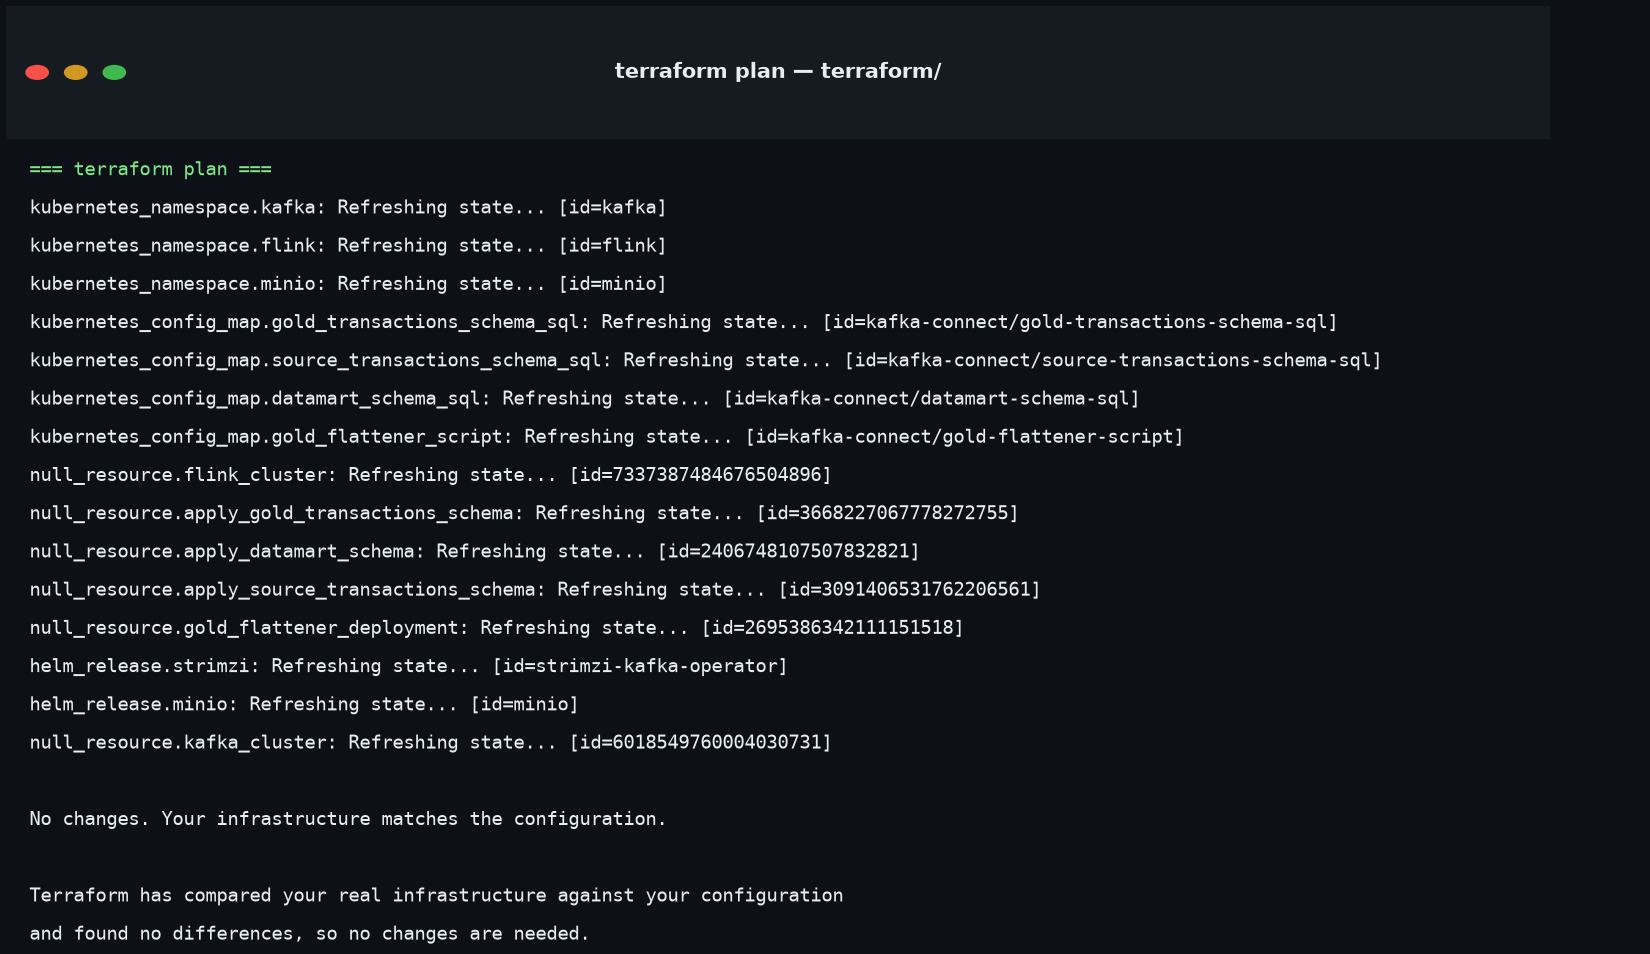
\includegraphics[width=0.95\textwidth]{figures/terraform-apply.png}
\caption{Provisionnement de l'infrastructure via Terraform}
\label{fig:terraform}
\end{figure}

\subsection{Pods Kubernetes en cours d'execution}

La figure \ref{fig:pods} liste l'ensemble des pods actifs, repartis sur les cinq
namespaces du cluster (\texttt{kafka}, \texttt{flink}, \texttt{minio},
\texttt{kafka-connect}, \texttt{monitoring}), tous a l'etat \texttt{Running}.

\begin{figure}[H]
\centering
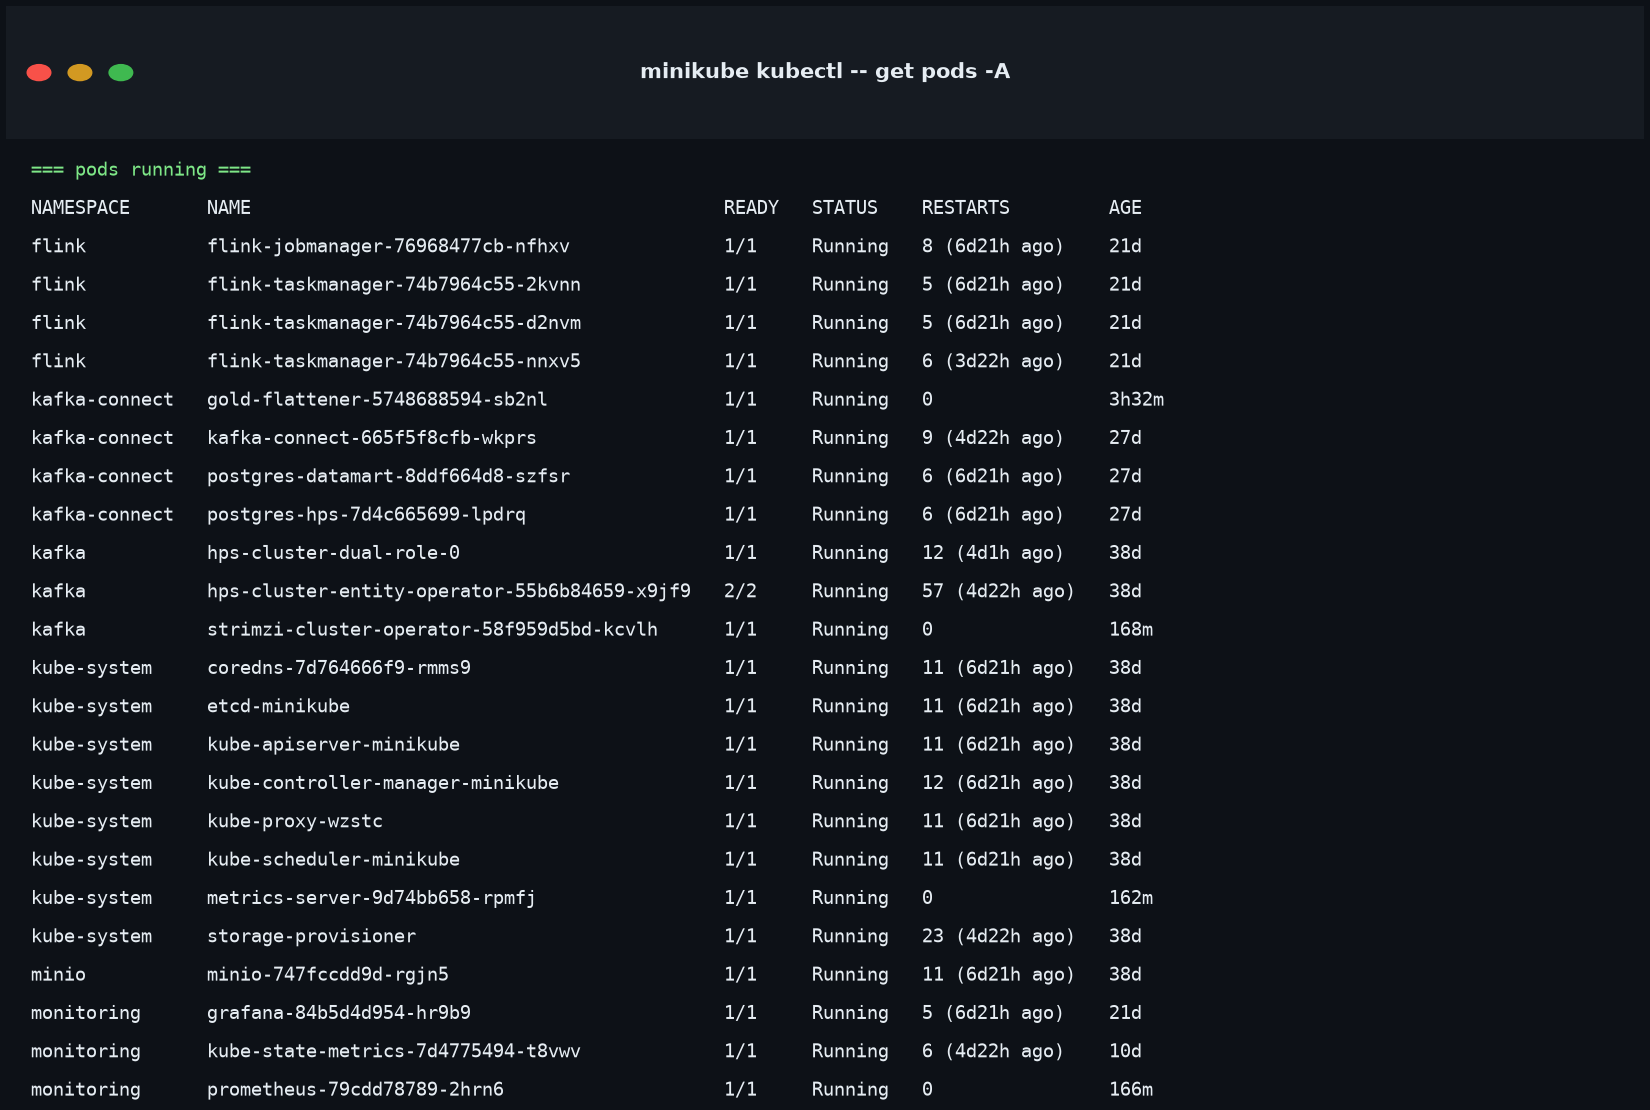
\includegraphics[width=0.95\textwidth]{figures/pods-running.png}
\caption{Etat des pods Kubernetes du pipeline}
\label{fig:pods}
\end{figure}

\subsection{Cluster Kafka}

La figure \ref{fig:kafka-cluster} confirme l'etat \texttt{Ready} du cluster Kafka
\texttt{hps-cluster}, gere par l'operateur Strimzi en mode KRaft.

\begin{figure}[H]
\centering
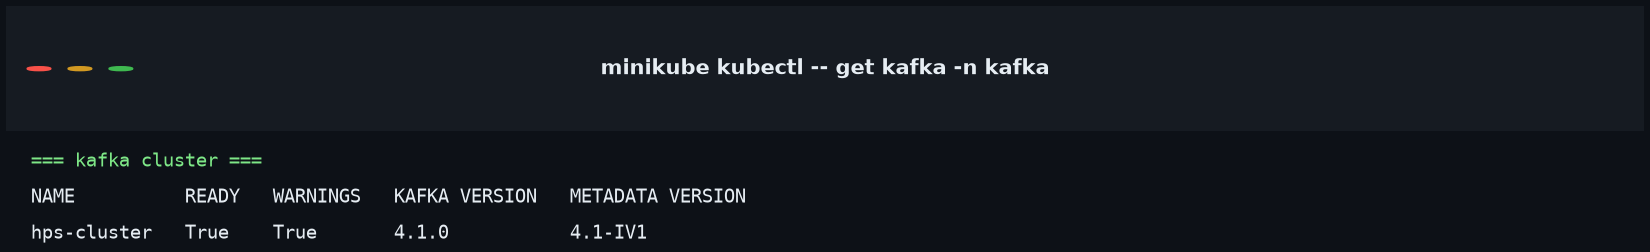
\includegraphics[width=0.8\textwidth]{figures/kafka-cluster.png}
\caption{Etat du cluster Kafka (Strimzi, mode KRaft)}
\label{fig:kafka-cluster}
\end{figure}

\subsection{Topics Kafka}

La figure \ref{fig:kafka-topics} liste les sept topics du pipeline, chacun a l'etat
\texttt{Ready}, avec leur nombre de partitions et leur facteur de replication.

\begin{figure}[H]
\centering
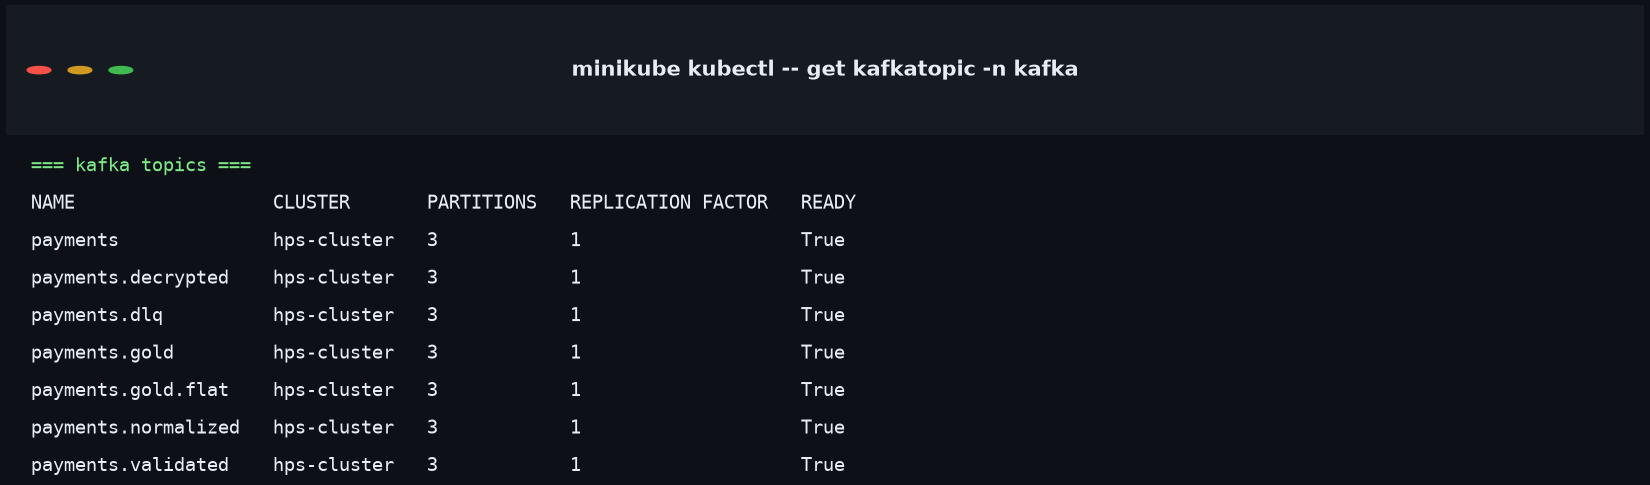
\includegraphics[width=0.95\textwidth]{figures/kafka-topics.png}
\caption{Topics Kafka du pipeline}
\label{fig:kafka-topics}
\end{figure}

\subsection{Tableau de bord Flink}

Le tableau de bord Flink (figure \ref{fig:flink-dashboard}) permet de superviser
l'execution des quatre jobs de traitement (decryptage, validation, normalisation,
optimisation), leur taux de traitement et l'etat de leurs checkpoints.

\figuremanquante{flink-dashboard.png --- capture du tableau de bord Flink (necessite
un navigateur, indisponible dans cet environnement d'execution)}

\subsection{Console MinIO}

La console MinIO (figure \ref{fig:minio-console}) permet de visualiser les trois
couches de l'architecture Medallion --- Bronze, Silver et Gold --- au sein du bucket
\texttt{rt-payments}.

\figuremanquante{minio-console.png --- capture de la console MinIO (necessite un
navigateur, indisponible dans cet environnement d'execution)}

\subsection{Connecteur Kafka Connect JDBC Sink}

La figure \ref{fig:debezium} presente l'etat du connecteur \texttt{gold-transactions-sink},
charge d'inserer chaque enregistrement de \texttt{payments.gold.flat} dans la table
\texttt{gold\_transactions} de PostgreSQL.

\begin{figure}[H]
\centering
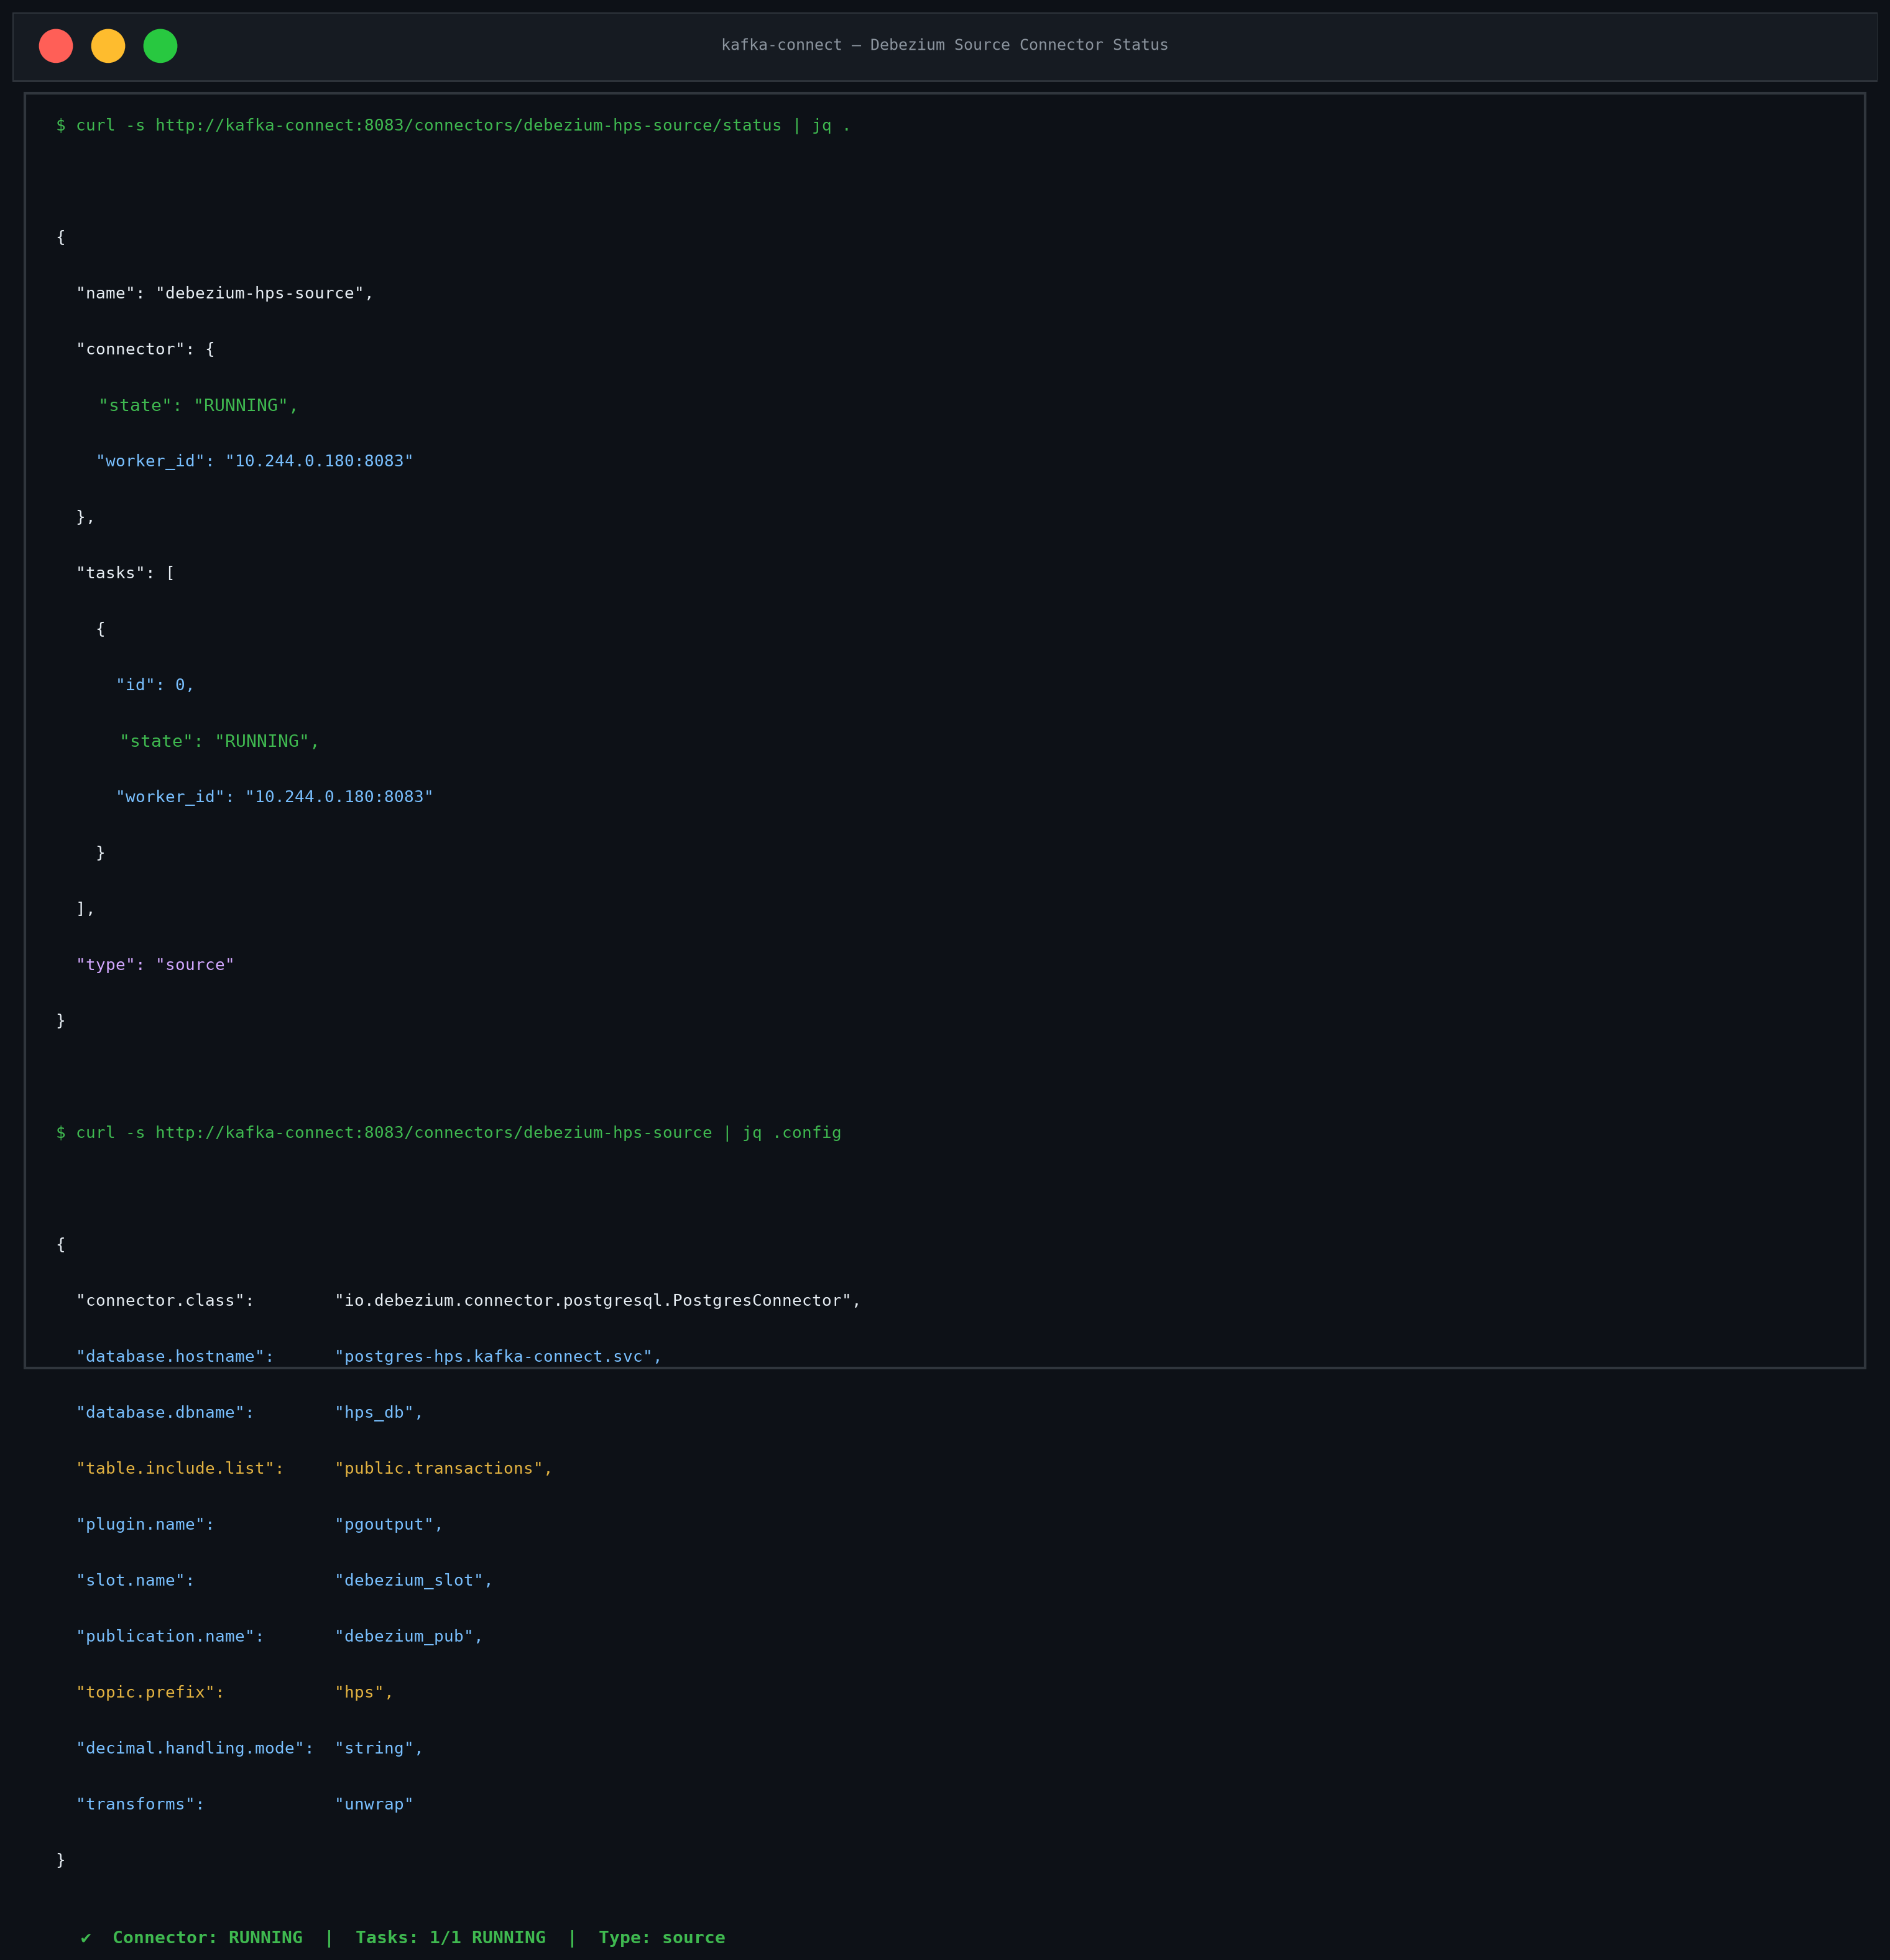
\includegraphics[width=0.95\textwidth]{figures/debezium-running.png}
\caption{Etat du connecteur Kafka Connect JDBC Sink}
\label{fig:debezium}
\end{figure}

\subsection{Donnees gold\_transactions}

La figure \ref{fig:datamart-rows} presente un extrait des enregistrements les plus
recents de la table \texttt{gold\_transactions}, alimentee en temps reel par le
pipeline.

\begin{figure}[H]
\centering
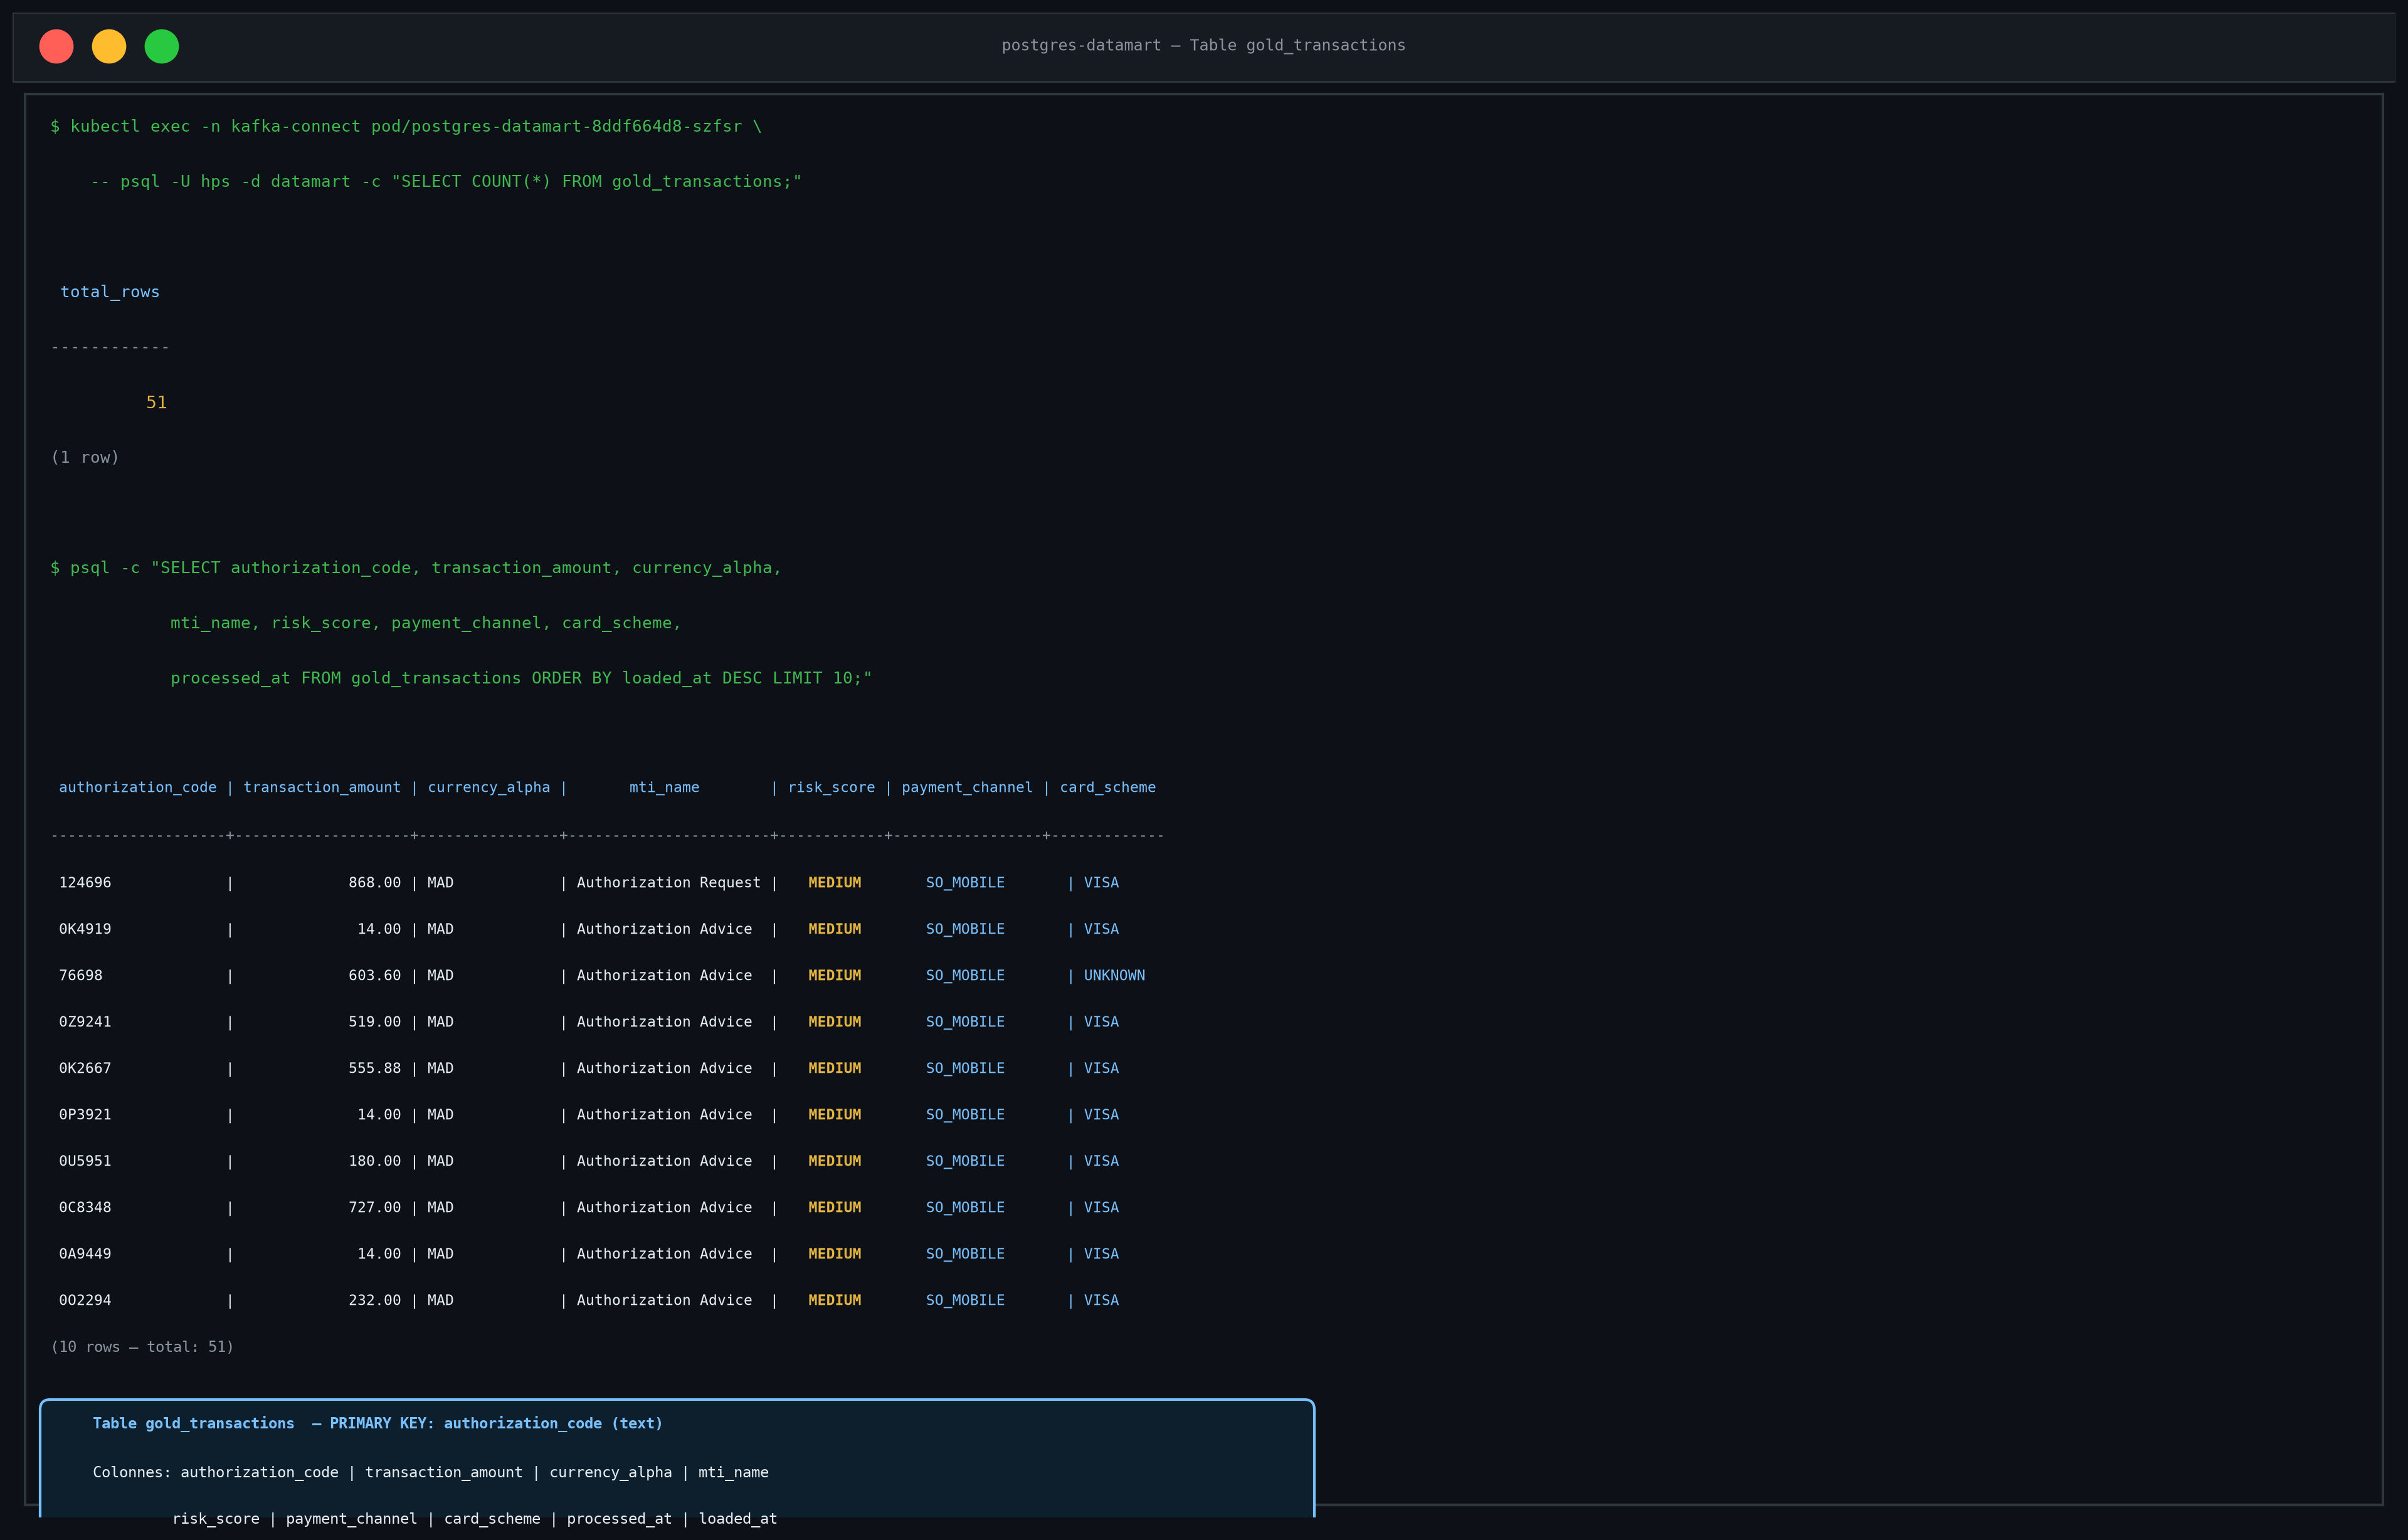
\includegraphics[width=0.95\textwidth]{figures/datamart-rows.png}
\caption{Extrait de la table gold\_transactions}
\label{fig:datamart-rows}
\end{figure}

\subsection{Tableau de bord Grafana}

Les tableaux de bord Grafana (figure \ref{fig:grafana}) restituent en temps reel les
metriques metier (volumes par etape, score de risque, canal de paiement) ainsi que les
metriques d'infrastructure (CPU, memoire, reseau par namespace).

\figuremanquante{grafana-dashboard.png --- capture d'un tableau de bord Grafana
(necessite un navigateur, indisponible dans cet environnement d'execution)}

\subsection{Cibles Prometheus}

La figure \ref{fig:prometheus} montre l'ensemble des cibles de collecte (\textit{targets})
configurees dans Prometheus, toutes a l'etat \texttt{UP}.

\figuremanquante{prometheus-targets.png --- capture de la page targets de Prometheus
(necessite un navigateur, indisponible dans cet environnement d'execution)}

\section{Validation globale du pipeline}
\label{sec:validation}

Un test de bout en bout a ete realise en injectant un lot de transactions via le
producteur Python. Le tableau \ref{tab:volumes} recapitule les volumes observes a
chaque etape du pipeline lors de cette validation.

\begin{table}[H]
\centering
\renewcommand{\arraystretch}{1.4}
\begin{tabular}{|l|r|}
\hline
\textbf{Etape / Topic} & \textbf{Nombre de messages} \\
\hline
\texttt{payments} (brut chiffre) & 496 \\
\texttt{payments.decrypted} & 575 \\
\texttt{payments.validated} & 766 \\
\texttt{payments.normalized} & 1068 \\
\texttt{payments.gold} & 368 \\
\texttt{payments.dlq} & 165 \\
\texttt{gold\_transactions} (PostgreSQL) & 50 \\
\hline
\end{tabular}
\caption{Volumes de donnees observes par etape du pipeline}
\label{tab:volumes}
\end{table}

\conclusionchapitre

Ce chapitre a presente la realisation concrete du pipeline, depuis le provisionnement
automatise de l'infrastructure jusqu'a la persistance finale des donnees enrichies,
en illustrant chaque etape par les interfaces et sorties produites par le systeme en
fonctionnement reel. L'ensemble des composants --- Kafka, Flink, MinIO, Kafka Connect,
PostgreSQL et la chaine de monitoring --- a ete valide de bout en bout.
